%\section{Electro-osmotic flow in a slit pore}
%Electro-osmotic flow (EOF) is the motion of water (or another liquid)
%induced by an electric field. It can occur e.g. in porous media,
%in synthetic capillaries and in vicinity of charged surfaces.
%Charged objects in an electrolyte solution attract ions of one
%species and repel ions of the other species, which gives rise
%to a net charge density in its neighbourhood. If an external
%electric field is applied, these ions are accelerated in the direction
%of the electric field (or oppositely if negatively charged) which
%causes also an acceleration of the surrounding water. In regions
%with zero net charge, the force on the fluid exerted by both ion
%species cancels, thus charged interfaces are necessary.
%
%Conceptually electro-osmotic flow is closely related to electrophoresis,
%where a charged object (e.g. a polyelectrolyte) is moved by an
%electric field and the surrounding counterions create a flow field
%in the opposite direction. 
%
%In this exercise the electrokinetic equations, that allow for a classical
%description of the phenomenon, are introduced and you will learn
%how to simulate this effect with \ES{} with the LBM. The special case of
%planar charged walls in the regime of low salt concentration can
%be solved analytically and you will see that we can reproduce the
%classical results quite well, but you will also learn about the
%deficiencies of both approaches. We will concentrate on the case
%where only one species of ions (counterions) is present. The generalization
%to multiple species however is straightforward.
%
%\subsection{The electrokinetic equations}
%We want to describe a system in which ions can diffuse under an
%applied field embedded in a fluid. We therefore assume that a 
%linear convection diffusion equation is valid:
%\begin{align*}
%		\vec j &=-D\nabla\rho-\rho\left(\mu z e \nabla\Phi+\vec u\right),
%\end{align*}
%
%Here $\vec{j}$ corresponds to the ion flux density, $D$ corresponds 
%to the diffusion coefficient of the ions,
%$\rho$ to their concentration, $\mu$ to their (electrophoretic)
%mobility, $z$ the valency, $\vec{E}$ to the local electric field and $\vec{u}$
%to the fluid velocity.
%
%We assume that the fluid fulfills the incompressible Navier-Stokes equation.
%The term $\rho z e \vec{E}$ appears as source term due
%to the acceleration of the fluid caused by the ions. 
%In the limit of small Reynolds numbers we can leave out
%the convection term and reduce to the Stokes equation.
%\begin{equation}
%  \eta \Delta \vec{u} = \vec{\nabla} p - \rho z e \vec{E}
%\end{equation}
%Here we have assumed that the system reaches a steady
%state and therefore the time derivative was dropped.
%The incompressibility (=continuity) equation holds:
%\begin{equation}
%  \vec{\nabla} \cdot \vec{u} = 0
%\end{equation}
%For the electrostatic potential we make the following
%mean field approximation: The electric potential is 
%caused not by single ions, but their density. This means
%every ion is not exposed to the instantaneous electrostatic potential
%but the smeared out potential of all other ions. Then the Poisson
%equation reads as:
%\begin{equation}
%  \Delta \Phi = -\rho z e/\varepsilon
%  \label{asdf}
%\end{equation}
%We will later
%see that this approximation is avoided in a molecular dynamics simulation
%of explicit ions.
%
%This set of coupled partial differential equations is called
%the electrokinetic equations. In general the solution is difficult,
%but the planar geometry will allow us to find an analytical 
%solution.
%
%\subsection{The slit pore geometry}
%We want to investigate the simplest case where EOF occurs:
%The flow of water through the volume between two parallel
%charged planes in the $xy$-plane. We assume that the planes are infinitely
%extended in the directions parallel to the plane and that
%the number of ions exactly cancels the charge of both planes
%and that the external electric field is exerted in $x$ direction
%and that the position of the planes is at $x=\pm l/2$.
%
%We assume that all quantities do not change in $y$ and $z$ directions
%because of translational invariance (the great advantage of our geometry)
%and drop all derivatives with respect to it. The only exception
%is the electrostatic potential which we assume to decay linearly in
%$y$-direction due to an external field. 
%
%
%Due to continuity in $x$-direction and translational invariance resp.
%symmetry the fluid velocity and flux density in x direction must be zero and we can 
%write down the Poisson equation and the diffusion equation in 
%$x$ direction:
%\begin{align}
%  \partial^2_x \Phi &= -\rho z e/\varepsilon \\
%	0 &=-D\partial_x\rho-\rho\mu z e \partial_x\Phi
%\end{align}
%This significantly smaller set of equations corresponds
%to the 1D Poisson-Boltzmann equation. It can be solved
%using the Ansatz:
%\begin{equation}
%  \rho = c \exp\left(-\frac{z e \Phi}{k_B T}\right)
%\end{equation}
%Then one obtains a single ordinary differential
%equation that has to be solved under the boundary 
%condition that the walls bear a charge density $\sigma$,
%thus electric field jumps at $x=\pm l/2$. This
%yields:
%\begin{align*}
%		\rho(y)=\frac{\varepsilon\,C^2}{2 k_B T}\cdot\frac 1 {\cos^2\left(\frac{qC}{2k_B T}\cdot y\right)},\quad \left|\frac{qC}{2k_B T}\cdot y\right|<\frac\pi 2\,.
%	\end{align*}
%Here the parameter $C$ has to fulfill the following transcendental
%equation:
%	\begin{align*}
%		C\cdot\tan\left(\frac{qd}{4k_B T}\cdot C\right)=-\frac\sigma\varepsilon,\quad 0\le C<\frac{\pi k_B T}{2d|q|}\,.
%	\end{align*}
%Now this charge density can be included in the Stokes equation
%and one can obtain the fluid profile from integrating twice
%and choosing the integration constanst so that $\vec u=0$ is fulfilled
%at $x=\pm l/2$:
%	\begin{align*}
%		u_y(x)&=\frac{2E\varepsilon k_B T}{\eta q}\cdot\left\{\log\left[\cos\left(\frac{qC}{2k_B T}\cdot x\right)\right]-\log\left[\cos\left(\frac{dqC}{4k_B T}\right)\right]\right\},\\
%	\end{align*}
%Obtaining the particle flux profile is the easy:
%\begin{equation}
%  j_y / \rho = \mu E + u_y.
%\end{equation}
%
%Before simulating the full system, we make two steps in between, because
%we need to know how to have walls in an \ES{} simulation. First we want
%to simulate Poisseuille flow, the famous parabolic flow profile, in a slit
%geometry and then we want to simulate particles between two walls. Finally
%we combine it all to simulate the full system.

\section{Poiseuille flow \ES{}}
Poisseuille flow is the flow through a pipe or (in our case) a slit
under a homogenous force density, e.g. gravity. In the limit of small Reynolds
numbers, the flow can be described with the Stokes equation. 
We assume the slit being infinitely extended in $y$ and $z$ 
direction and a force density $f$ on the fluid 
in $y$ direction. No slip-boundary conditions  (i.e. $\vec{u}=0$)
are located at $z = \pm l/2$.
Assuming invariance in $y$ and $z$ direction and a steady state 
the Stokes equation is simplified to:
\begin{equation}
  \eta \partial_x^2 u_y = f
\end{equation}
where $f$ denotes the force density and $\eta$ the dynamic viscosity.
This can be integrated twice and the integration constants are chosen
so that $u_y=0$ at $z = \pm l/2$ and we obtain:
\begin{equation}
  u_y = \frac{f}{2\eta} \left(l^2/4-x^2\right)
\end{equation}
With that knowledge investigate the script \texttt{poisseuille.py}.
Note the use of the \texttt{lbboundaries} module. Two walls are created
with normal vectors $\left(\pm 1, 0, 0 \right)$. An external force
is applied to every node. After 5000 LB updates the steady state should
be reached.

Task: Write a loop that prints the fluid velocity at the nodes (0,0,0) to (16,0,0)
and the node position to a file. Use the \texttt{lbf.[node].quantity}
method for that. Hint: to write 
to a file, first open a file and then use the \texttt{write()} method to write 
into it. Do not forget to close the file afterwards. Example:
\vspace{ 0,2cm}
\begin{pypresso}
f = open("file.dat", "w")
f.write("Hello world!\n")
f.close()
\end{pypresso}
\vspace{ 0,2cm}
Use the data to fit a parabolic function. Can you confirm the analytic solution?
\begin{figure}[h]
  \begin{center}
    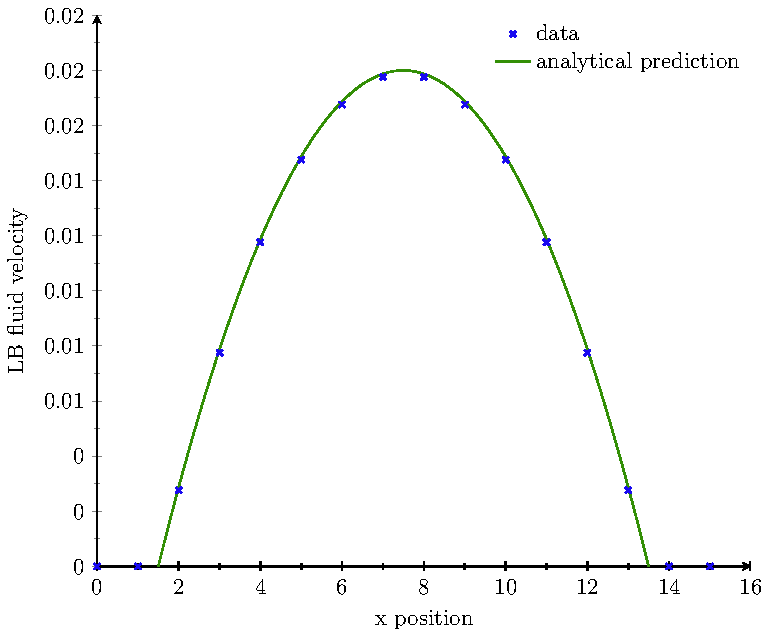
\includegraphics{figures/poiseuille/poiseuille.pdf}
  \end{center}
  \caption{Poisseuille Flow in a slit Geometry.}
\end{figure}

%\subsection{Constraints in \ES{}}
%The \lstinline|constraint| command of \ES{} creates walls in the system.
%They have a particular ``particle'' type and interact with the particles
%present in the system with the potential defined 
%between them. This means the distance
%of every particle to the constraint is calculated and used as the distance 
%in the interaction potential.
%
%To set up a planar channel like the LB channel before one would use the commands:
%\begin{lstlisting}[numbers=none]
%constraint wall dist 0.5 normal 1. 0. 0. type 1
%constraint wall dist -8.5 normal -1. 0. 0. type 1
%inter 0 1 lennard-jones 1. 1. 1.225 0.25 0
%\end{lstlisting}
%This wall is felt only by particles of type 0 and has an effective width
%of 6, as the potential goes steeply up at positions $x=1.5$ and $x=7.5$.
%
%The syntax of the wall constraint looks weird at first, because a negative
%distance from the origin (first argument) is given, but the idea is that
%this distance times the normal vector is a point of the plane. For inclined
%walls this syntax is more easy to understand.
%
%\ES{} complains every time a particle penetrates the wall, as it does not
%expect the particles to do so. This complaint should be taken serious, because
%that means the particle has overcome LJ potential barrier, which is physically
%impossible. This usually tells you to reduce the applied time step.
%
%To set up a system we have, of course to make sure, that our initial
%configuration obeys the constraints. The easiest thing is to 
%generate particle positions randomly and check if it obeys the constraint.
%If not we repeat this process
%for every particle until a configuration is found, that
%is within the allowed range. Look at the script \lstinline|boundaries.tcl|
%and see how that is solved. What does the script do?
%Introduce an LB fluid with planar walls boundaries at 2.5 and 12.5. 
%\subsection{Simulating EOF in \ES{}}
%The last thing that is missing for the simulation of EOF is
%how to create a charged wall. This can be done with
%particles, using the \lstinline|fix| command. The command
%\begin{lstlisting}[numbers=none]
%part 0 pos 1. 1. 1. q 1. fix 1 1 1
%\end{lstlisting}
%create a particle at the position $\left(1,1,1\right)$ with
%charge 1 that is fixed in all the spacial dimensions.
%
%In \lstinline|eof.tcl| two walls are created. Now use the material
%from the other two scripts to run the final system.
%We want to obtain a 10 Nanometer wide channel centered
%$x=7.5$
%\begin{enumerate}
%  \item Create constraints at $x=1.5$ and $x=13.5$ and create 
%    a particle-wall interaction. How can you assure that the 
%    particles creating the wall charges are not affected by 
%    interaction potential?
%  \item
%Use the particle
%creation method from \lstinline|boundaries.tcl| to
%create particles in the system. Create a repulsive potential between them.
%  \item
%Charge the particles so that
%the overall system is neutral. 
%  \item Add an electrostatic interaction with a Bjerrum length 
%    of 0.7 (the room temperature Bjerrum length of water in nanometer).
%  \item First do not exert an external force on the particles.
%       Use a Langevin thermostat to bring the system to equilibrium.
%       It will take some time for the ions to move towards the charged
%       walls. You can use vmd to look at the process.
%  \item
%	  Use the density profile method from {\tt boundaries.tcl}
%       to determine the ion concentration profile. How many samples
%       do you need to get a reasonable concentration profile?
%   \item
%     Plot the concentration profile with gnuplot. Compare with the
%     the Poisson-Boltzmann result. 
%   \item 
%     Introduce an LB fluid with planar walls boundaries at 2.5 and 12.5. 
%     Do not forget to remove the
%	 external force if you copy\&paste from {\tt poisseuille.tcl}.
%   \item 
%     Add an external force of 0.1 to all particles that do not form the
%     charged wall in $y$-direction. Now run the system for enough time
%     steps to get a good flux and velocity profile.
%   \item 
%     Finally calculate the velocity profile. You will have to 
%     average over several steps. Keep in mind that number crunching
%     with tcl is slow and that you will not need to average over too 
%     many samples.
%   \item 
%     Compare the flux and velocity profiles with the result from
%     theory. Do they agree?
%   \item
%     Now increase the charge density on the walls. Can you observe differences
%     between theory and Computer simulations? They will likely be caused
%     by the fact, that MD simulations of explicit ions automatically
%     take into account ion correlations and the effect of the finite size
%     of ions.
%\end{enumerate}
%Following this list should in principle enable you to simulate the system. However
%we have figured out that quite some traps are on the way to the full system. You might
%have to make warmup steps in between, play with the time step and so on until your
%simulation script is really stable. If something happens, make sure you check all
%the stages in between, or make simplifications e.g. disabling the electrostatic interactions.
%This is however part of the process 
%to learn \ES{}. If it takes you some time, do not be disappointed, but 
%consider it a part of your learning curve.
%
%
%
%
%
%
%
%
%
%
%
%
%
%
%
